\documentclass[../../main]{subfiles}

\renewcommand\thesection{\arabic{section}}


\begin{document}

\section{Top and Side Hatches} \label{sec:}

As the seedlings mature and become ready for outdoor planting, it’s important
to gradually acclimate them to the external environment. The top hatch
facilitates this process by allowing controlled exposure. Additionally, the
side hatch provides convenient access for manual intervention when needed,
ensuring the user can easily tend to the seedlings. Refer figure \ref{fig:topHatch},
and \ref{fig:sideHatch} for the exact placement of these hatches.

\begin{center}

    \begin{tabularx} {\textwidth} {
            >{\centering \arraybackslash}X
            >{\centering \arraybackslash}X
        }

        \toprule

        Top Hatch & Side Hatch \\

        \midrule

        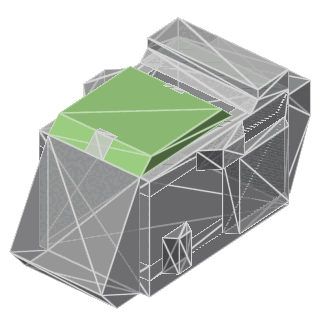
\includegraphics [
            height = 0.18\textheight,
        ] {pics/top_hatch_right.png}

        &

        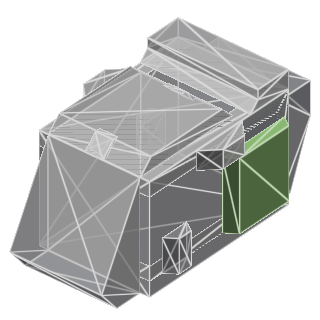
\includegraphics [
            height = 0.18\textheight,
        ] {pics/side_hatch_right.png}

        \\
        \vspace{-0.5cm}

        \captionof{figure}[CAD rendering of top hatch.]{}
        \label{fig:topHatch}

        &

        \vspace{-0.5cm}
        \captionof{figure}[CAD rendering of side hatch.]{}
        \label{fig:sideHatch}

        \\

        \bottomrule

    \end{tabularx}

\end{center}

\subsection{Hatch Control}

There are several ways to control the opening and closing of these
hatches. One way is to use stepper motors. The other way is to use geared
DC motors with some form of feedback for the position of the hatch panels.
Both the top and side hatch panels are made of foam, so weight won't be
an issue. Since we've already bought some geared DC motor as part of
mini project, we are going to drive these panels using them.

\subsection{Hatch Feedbacks}

Since we are using DC motors we cannot accurately single step them. We
need to find some other way to know the current position of each of the panels.
Something like a linear potentiometer will be perfect for this case. But commercial
ones are really expensive. So we need to make a home brew one. Along with
linear potentiometer, we will be using limit switches.

\alertNote{
    The hatch control will be mediated by the main boards of the auxiliary system, and
    the feedback will be read through one of the multiplexer boards.
}

\alertWarning{
    Design for these hatches, that is the mechanical design, controlling circuits,
    and feedback mechanisms are still in its infancy.
}

% interfacing circuits

\end{document}
